% ===================================SBAI==================================
\documentclass[a4paper]{ifacconf}
\usepackage{graphicx,amsmath,url}      % include this line if your document contains figures
\usepackage[round]{natbib}             % required for bibliography
\usepackage[spanish,brazil,english]{babel}
\usepackage[T1]{fontenc}
%\usepackage{inputenc}
\usepackage[utf8]{inputenc}
\usepackage{ae}
\newtheorem{teorema}[thm]{{\em Teorema}}{ }
\newtheorem{lema}[thm]{{\em Lema}}{ }
\newtheorem{corolario}[thm]{{\em Corolário}}{ }
\newenvironment{prova}{{\bf Prova.}}{ }

% ===========================PACOTES==ADICIONAIS==AQUI======================
%\usepackage[utf8]{inputenc}
%\usepackage{float}
%\usepackage{ae}
%\usepackage{amsfonts, amssymb}
%\usepackage{amsmath}
%\usepackage{graphicx}
%\usepackage{indentfirst}
%\usepackage{ae}
%\usepackage{gensymb}
%\usepackage{caption} 
\usepackage{epstopdf}
%\usepackage{leading}
%\makeatletter
%\def\verbatim@font{\normalfont\ttfamily\footnotesize}
%\makeatother
%\usepackage{amsmath}
\usepackage{hyperref}
\usepackage{float}

\begin{document}
    \selectlanguage{brazil}
	
\begin{frontmatter}
    
    % Title, preferably not more than 10 words.
    %\title{Implementação de um Arranjo Cliente Servidor para um Robô Industrial com Controladora Aberta}
    \title{Arranjo Cliente Servidor para um Robô Industrial com Controladora Aberta}  
    
    %\thanks[footnoteinfo]{Reconhecimento do suporte financeiro deve vir nesta nota de rodapé.}
    
    \author[First]{Thalles Oliveira Campagnani}  \author[First]{Renato de Sousa Dâmaso}
    
    \address[First]{Depto. de Eng. Mecatrônica do CEFET-MG, Unidade de Divinópolis 
    (thallescampagnani@gmail.com;  renatosd@cefetmg.br)}
    
    \selectlanguage{english}
    \renewcommand{\abstractname}{{\bf Abstract:~}}
    
    \begin{abstract}                % Abstract of not more than 250 words.
        This article describes the implementation of a software server, called OpenSever, in an industrial robotic system to facilitate the implementation of external control loops. The robotic system used is composed of an open controller, an external industrial computer and an industrial robotic manipulator. The open controller allows receiving movement commands from software compiled on the industrial computer, making use of the \textit{eORL} library. But this system is limited to the computational capacity of the industrial computer, its architecture \textit{x86}, its operating system based on \textit{Linux}, the programming language C/C++, which the library \textit{eORL} is compatible, and connection via cables. In order to overcome the aforementioned limitations, this software server was implemented in the industrial computer to enable the sending of movement commands by a software client on an external device. Such device can be of any architecture, operating system and programmed in any preferred language, as long as it has the ability to communicate with the server via the TCP/IP protocol through the network cable or wireless connection, and can do so use of simple open source operating system libraries. Once implemented, tests were carried out with some architectures, operating systems and programming languages. Some of the collected results are presented at the end.

        \vskip 1mm% não altere esse espaçamento
        \selectlanguage{brazil}
        {\noindent \bf Resumo}:  O presente artigo descreve a implementação de um software servidor, chamado OpenSever, num sistema robótico industrial para facilitar a implementação de malhas de controle externas. O sistema robótico utilizado é composto por uma controladora aberta, um computador industrial externo e um manipulador robótico industrial. A controladora aberta permite o recebimento de comandos de movimentação vindos de softwares compilados no computador industrial fazendo uso da biblioteca \textit{eORL}. Mas este sistema é limitado à capacidade computacional do computador industrial, a sua arquitetura \textit{x86}, ao seu sistema operacional baseado em \textit{Linux}, à linguagem de programação C/C++, que a biblioteca \textit{eORL} é compatível, e à conexão via cabos. A fim de superar as limitações citadas, foi implementado esse software servidor no computador industrial para possibilitar o envio de comandos de movimentação por um software cliente em um dispositivo externo. Tal dispositivo pode ser de qualquer arquitetura, sistema operacional e programado em qualquer linguagem de preferência, desde que tenha a capacidade de se comunicar com o servidor pelo protocolo TCP/IP através do cabo de rede ou conexão sem fio. Além disso, podendo fazer uso de bibliotecas simples de código aberto do sistema operacional. Depois de implementado, foram feitos testes com algumas arquiteturas, sistemas operacionais e linguagens de programação. Ao final, são apresentados alguns dos resultados coletados.

    \end{abstract}
    
    \selectlanguage{english}
    \begin{keyword}%Five to ten keywords separatety by semicolon. 
        C5G Open, Industrial Robotic Manipulator, Client server arrangement
        \vskip 1mm% não altere esse espaçamento
        \selectlanguage{brazil}
        {\noindent\it Palavras-chaves:} C5G Open, Manipulador Robótico Industrial, Arranjo cliente servidor
        \end{keyword}
    
    \selectlanguage{brazil}

\end{frontmatter}

    \section{Introdução}
    Os robôs industriais tradicionais possuem uma arquitetura de controle fechada fornecida pelo fabricante. Esse tipo de solução segue o paradigma a qual deve ser priorizada a robustez e confiabilidade do funcionamento e da execução das tarefas, além de atender a certos requisitos normativos e legais que regem as indústrias. No entanto, é inegável que essa forma dificulta a realização de novas implementações e atividades de pesquisa com os mesmos.
    
    Algumas tentativas feitas pela academia foram relatadas na literatura no sentido de abrir a estrutura de controle de alguns robôs industriais~\citep{ROBERTI:2010}. Recentemente, alguns fabricantes de robôs perceberam essa demanda por parte das instituições de ensino e pesquisa e de forma semelhante ao que vem acontecendo com os softwares de código aberto do \textit{ROS} (Sistema Operacional Robótico, em tradução livre), oferecem a opção de abertura do sistema de controle de robôs~\citep{KUBUS:2010}, isto é, uma controladora aberta. 
    
    Uma opção para atender essa demanda foi desenvolvida pelo fabricante de robôs industriais \textit{Comau}, adicionando uma arquitetura complementar à controladora de seus robôs, a \textit{Comau C5G}. Essa extensão, denominada \textit{Comau C5G Open Controller}, é feita através da conexão da controladora a um computador industrial externo, denominado \textit{LPC (Linux Personal Computer)}, como é mostrado na Figura~\ref{controladora2}.~\citep{ANTONELLI:2010}.
    
    A Figura~\ref{controladora} permite a visualização da solução fornecida pelo fabricante, sendo que, a conexão \textit{Ethernet} TCP-IP precisa ser intermediada por um modem, roteador ou \textit{switch} não fornecido nessa extensão.
    \begin{figure}[ht]
        \centering
        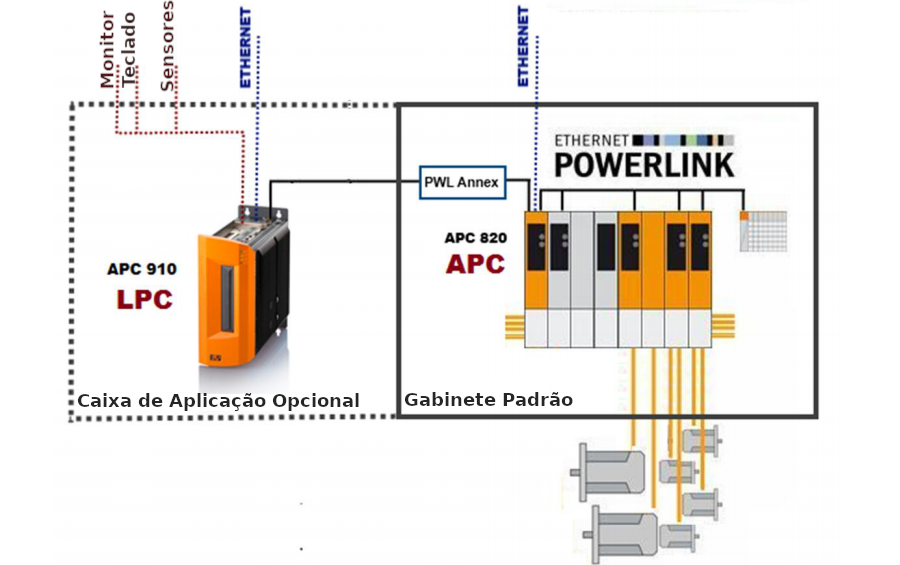
\includegraphics[width=\columnwidth]{imagens/Conexoes/controladora2.png}
        \small 
        \centering 
        \caption{Visão geral sobre o hardware do sistema C5G-Open}
        Adaptado de~\citep{Ferrara:2013}
        \label{controladora2}
    \end{figure} 
    
    Assim, é possibilitado à controladora do robô industrial enviar dados sensoriais e receber comandos de movimentação de um software a ser programado pelo usuário, a taxas de até 1 pacote a cada $0,4\,\mathrm{ms}$ (1 pacote contém todas as leituras de sensores do robô). Isso possibilita a criação de softwares que implementem malhas de controle adicionais como: controle de força, visão computacional, entre outros.~\citep{Ferrara:2013}
    
    \begin{figure}[ht]
        \centering
        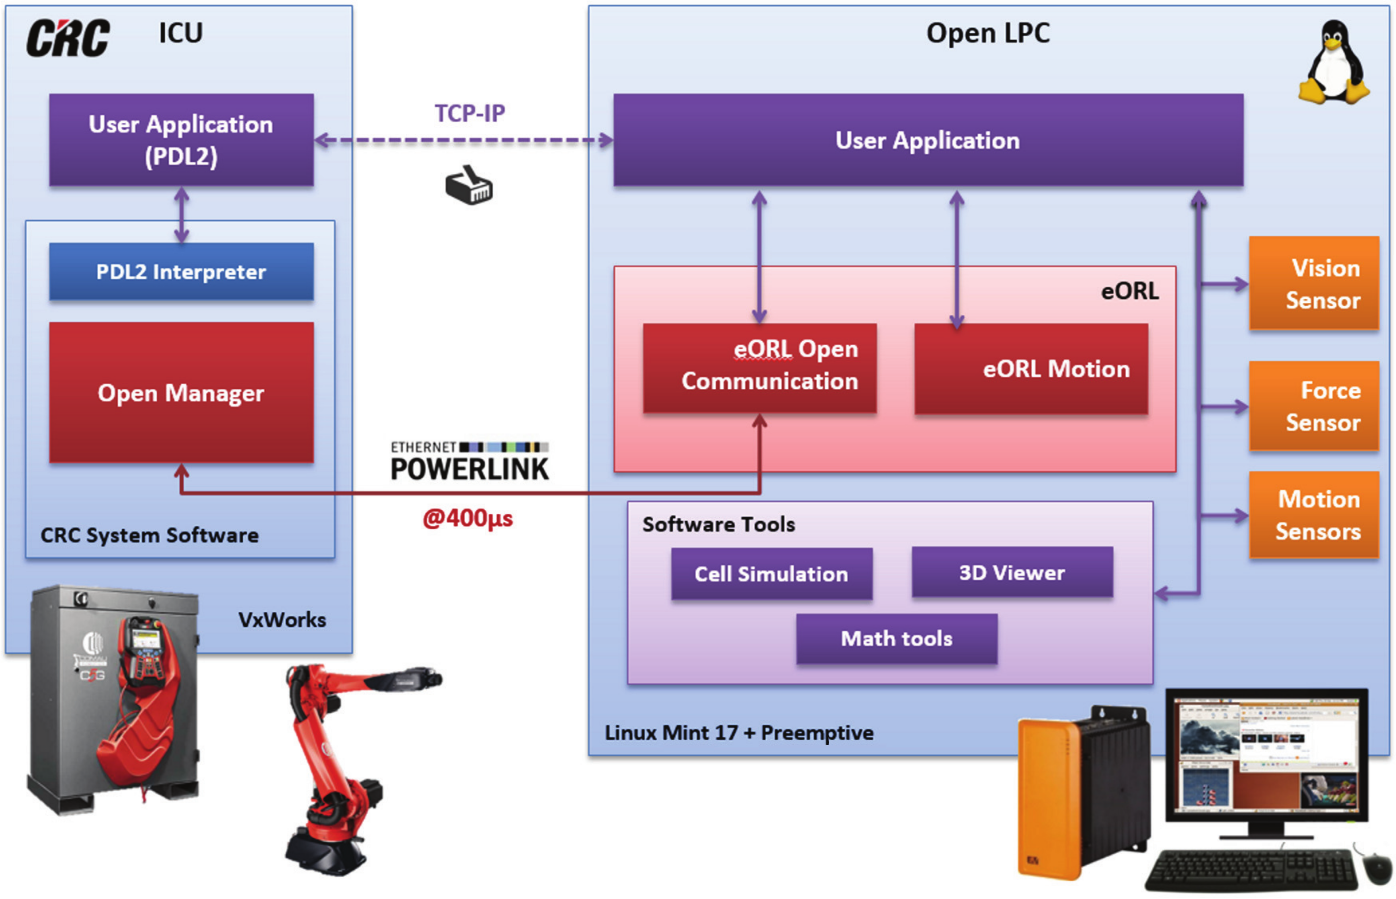
\includegraphics[width=\columnwidth]{imagens/Conexoes/controladora.png}
        \small 
        \centering 
        \caption{Visão geral do software do sistema C5G-Open}
        Fonte:~\citep{Open:Manual}
        \label{controladora}
    \end{figure} 
    
    Entretanto, existem algumas limitações, por exemplo: o software (\textit{User Application} na Figura \ref{controladora}) que implementa essa malha de controle adicional precisa ser compilado e executado nesse computador industrial externo, rodando o sistema operacional \textit{Linux Mint 17} compilado para arquitetura x86, conectado à controladora por um cabo de rede especial chamado \textit{Ethernet PowerLink} (visto na Figura \ref{controladora}). Ele precisa ser programado em C/C++ e utilizar a biblioteca proprietária de código fechado desenvolvida pela \textit{Comau} chamada \textit{eORL} (Biblioteca Robótica Realística Melhorada, em tradução livre) para controlar a comunicação.
    
    Além disso, uma utilização inadequada por um usuário que deixe a conexão com o \textit{LPC} habilitada do lado da controladora e que não tenha a adequada resposta do lado do \textit{LPC}, por exemplo, poderá produzir um erro de comunicação que acabará sendo armazenado em seus registros e impedirá a liberação dos \textit{drivers} da controladora pelo seu módulo de gerenciamento de segurança, chamado C5G-SDM (Módulo de Distribuição e Segurança, em português)~\citep{C5G:Manual}.
    
    Por fim, nem todos os programas necessários para o desenvolvimento de aplicações podem ser instalados no \textit{LPC}, como é o caso do \textit{ROS}, devido ao fato que os drivers do Powerlink Card precisam de uma versão mais antiga do Sistema Operacional Ubuntu (ou derivados dele, como Linux Mint) para funcionar~\citep{Bisson:2014}. Atualmente é executado no \textit{LPC} a versão 17 do Linux Mint, que é baseado na versão LTS (suporte de longa duração, em tradução livre) de 2014 do Ubuntu. Então, todos os programas e versões de bibliotecas do sistema operacional são versões ultrapassadas e, geralmente, não oferece suporte à instalação das novas versões dos mesmos, como é o caso do \textit{ROS 2}, que é a mais nova versão do \textit{ROS}.
    
    Visando oferecer mais liberdade e flexibilidade para o usuário, no que diz respeito à programação da malha de controle adicional e ao dispositivo que irá executá-la, foi desenvolvido um software chamado OpenServer. Este, tem também o objetivo de trazer mais segurança para a controladora do robô do laboratório do CEFET-MG em Divinópolis durante a execução de malhas de controle experimentais. Ele utiliza a biblioteca \textit{eORL} para controlar o robô e oferece uma \textit{API} (Interface de Programação de Aplicativo, em tradução livre) baseada em rede TCP/IP, o qual permite que um programa cliente em outro dispositivo controle o robô através dele. Este programa cliente pode ser escrito em qualquer linguagem de programação, compilado em qualquer arquitetura e executado em um sistema operacional de preferência. O OpenServer permite que o programa cliente leia os sensores do robô e envie os ângulos de referência para a controladora, possibilitando que o robô seja controlado até mesmo por aplicativos de \textit{smartphone} que utilizem a \textit{API}.
    
    Como mencionado acima, acredita-se que essa abordagem possa reduzir riscos ao equipamento por erro ou imperícia ao ser programada uma malha de controle usando recursos do sistema \textit{Open} fornecidos pelo fabricante. Pois, o OpenServer é programado para continuar se comunicando com a controladora, mesmo que a conexão com o programa cliente seja perdida. Além disso, ela é capaz de oferecer uma alternativa de \textit{API} mais simples de ser aprendida e utilizada.
    %na referida instituição de ensino.
    \section{O OpenServer}
    
    Para desenvolver o OpenServer foi aproveitada a estrutura padrão do sistema fornecida pela empresa fabricante, como detalhado na Figura~\ref{conexoes-padrao}, onde: (1) é a conexão elétrica entre Controladora e Manipulador Robótico; (2) representa a conexão \textit{PowerLink} entre \textit{LPC} e controladora; (3) é a conexão entre roteador e controladora; e (4) conexão entre roteador e o \textit{LPC}.

    \begin{figure}[ht]
        \centering
        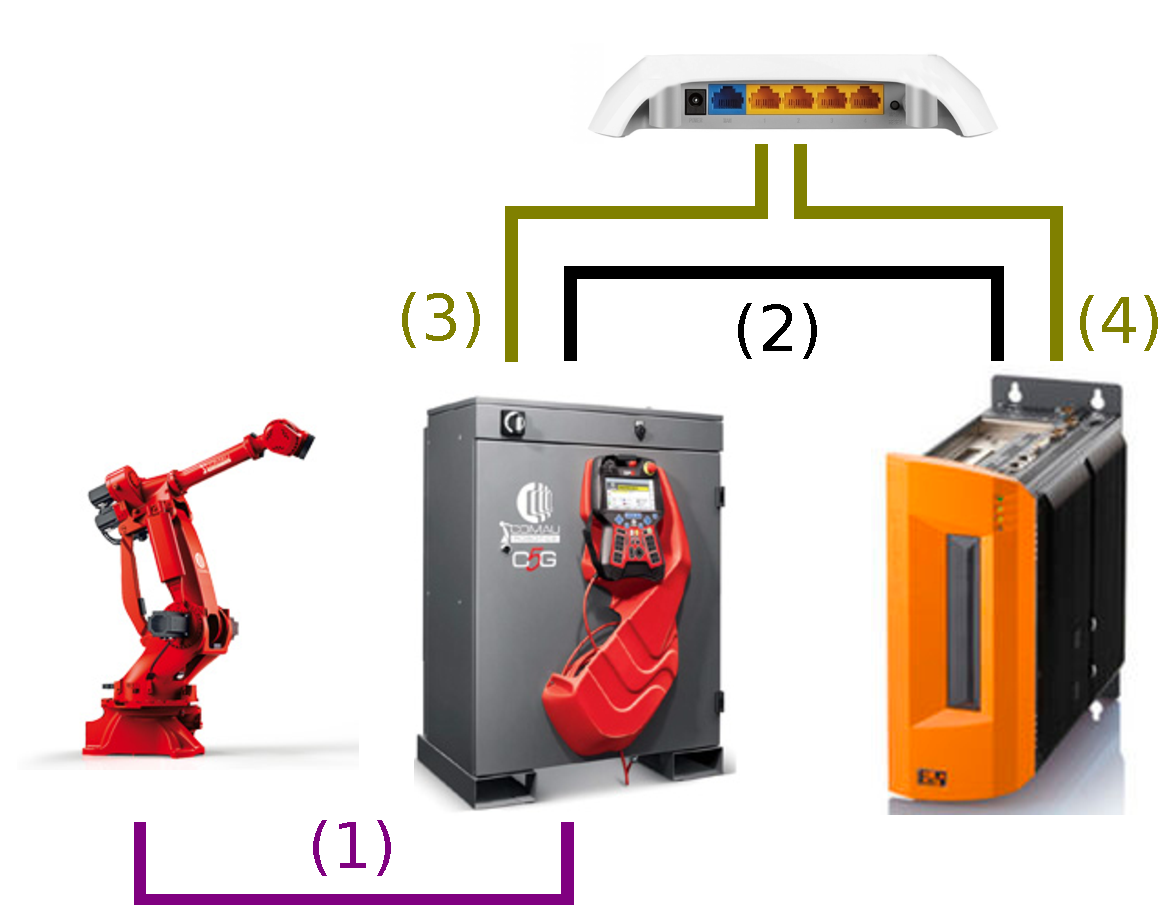
\includegraphics[width=\columnwidth]{imagens/Conexoes/conexoes-padrao.eps}
        \small 
        \centering 
        \caption{Estrutura padrão do sistema C5G Open}
        
        \label{conexoes-padrao}
    \end{figure}
      
    O OpenServer é um software do tipo servidor que permite o desenvolvimento de programas clientes que recebam por ele os dados sensoriais vindos da controladora do robô e envie através dele os comandos de movimentação para a mesma. No entanto, essa comunicação passará a ser feita usando uma rede \textit{Ethernet} convencional, através do uso do protocolo TCP/IP. Isso permite que o programa cliente possa ser programado na linguagem de programação de preferência do usuário, rodando em uma arquitetura e sistema operacional disponíveis.
    
    Para isso, o OpenServer foi programado dentro das limitações da plataforma, ou seja, na linguagem C++ usando a biblioteca \textit{eORL} do fabricante do robô, usando a rede \textit{PowerLink} para fazer a comunicação com a controladora do robô e sendo compilado para o sistema operacional baseado em Linux com arquitetura x86. Além disso, ele usa bibliotecas padrão em C++ disponíveis para o sistema operacional \textit{Linux Mint} para realizar a comunicação via rede TCP/IP. A estrutura desenvolvida para execução do OpenServer passa então a ser conforme mostra a Figura~\ref{conexoes-openserver}, onde: (5) representa a conexão entre o roteador e o dispositivo externo, a qual, pode ser feita através de cabeamento ou conexão sem fio; e (6) é a conexão entre roteador e rede institucional.
    
    \begin{figure}[ht]
        \centering
        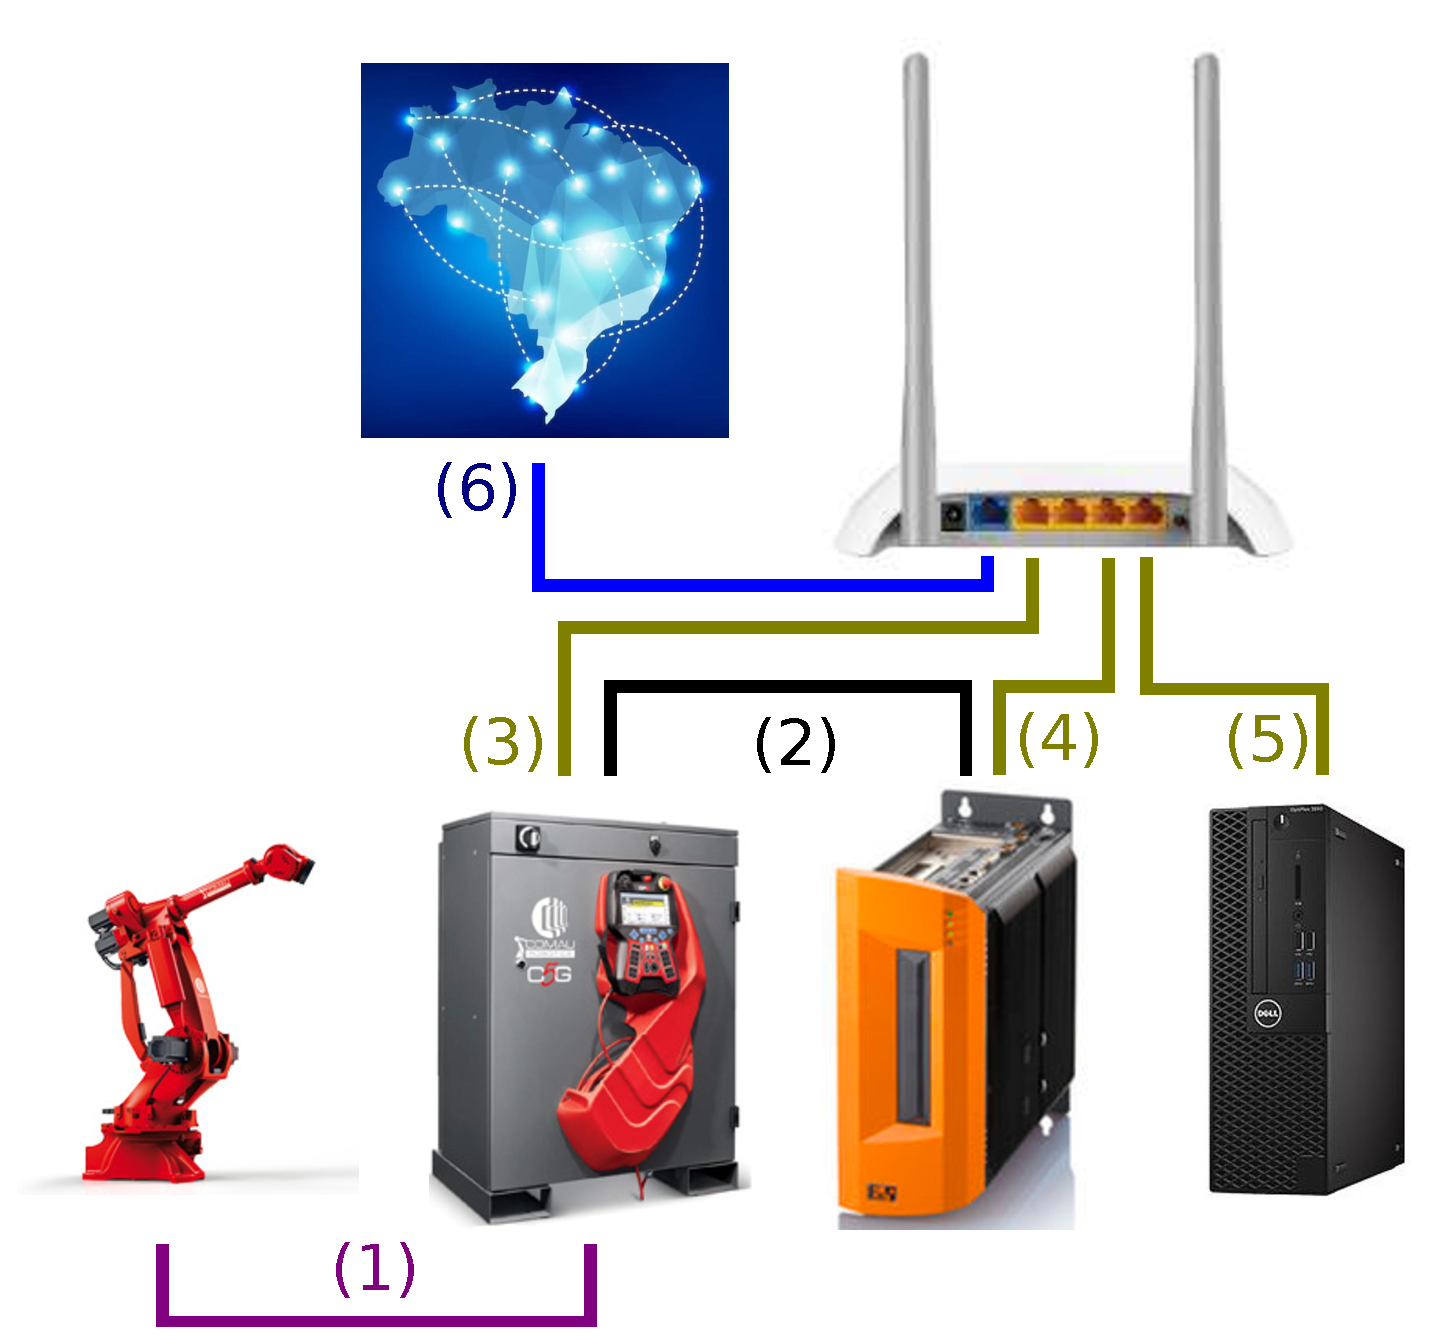
\includegraphics[width=\columnwidth]{imagens/Conexoes/conexoes-openserver.eps}
        \small 
        \centering 
        \caption{Estrutura desenvolvida para execução do OpenServer}
        
        \label{conexoes-openserver}
    \end{figure}
    
    
    A rede institucional do CEFET-MG oferece acesso à internet. No entanto, as portas do roteador são bloqueadas para acesso externo. Dessa forma, é criada uma rede interna segura onde os softwares são executados. Por esta razão, não foram implementadas soluções de criptografia de dados, bem como de autenticação. Isso ocorreu também pelo motivo de ser um ambiente acadêmico, controlado e sem trafego de dados sensíveis. A estrutura real do sistema pode ser visto na Figura~\ref{lab1}.
    
    \begin{figure}[ht]
        \centering
        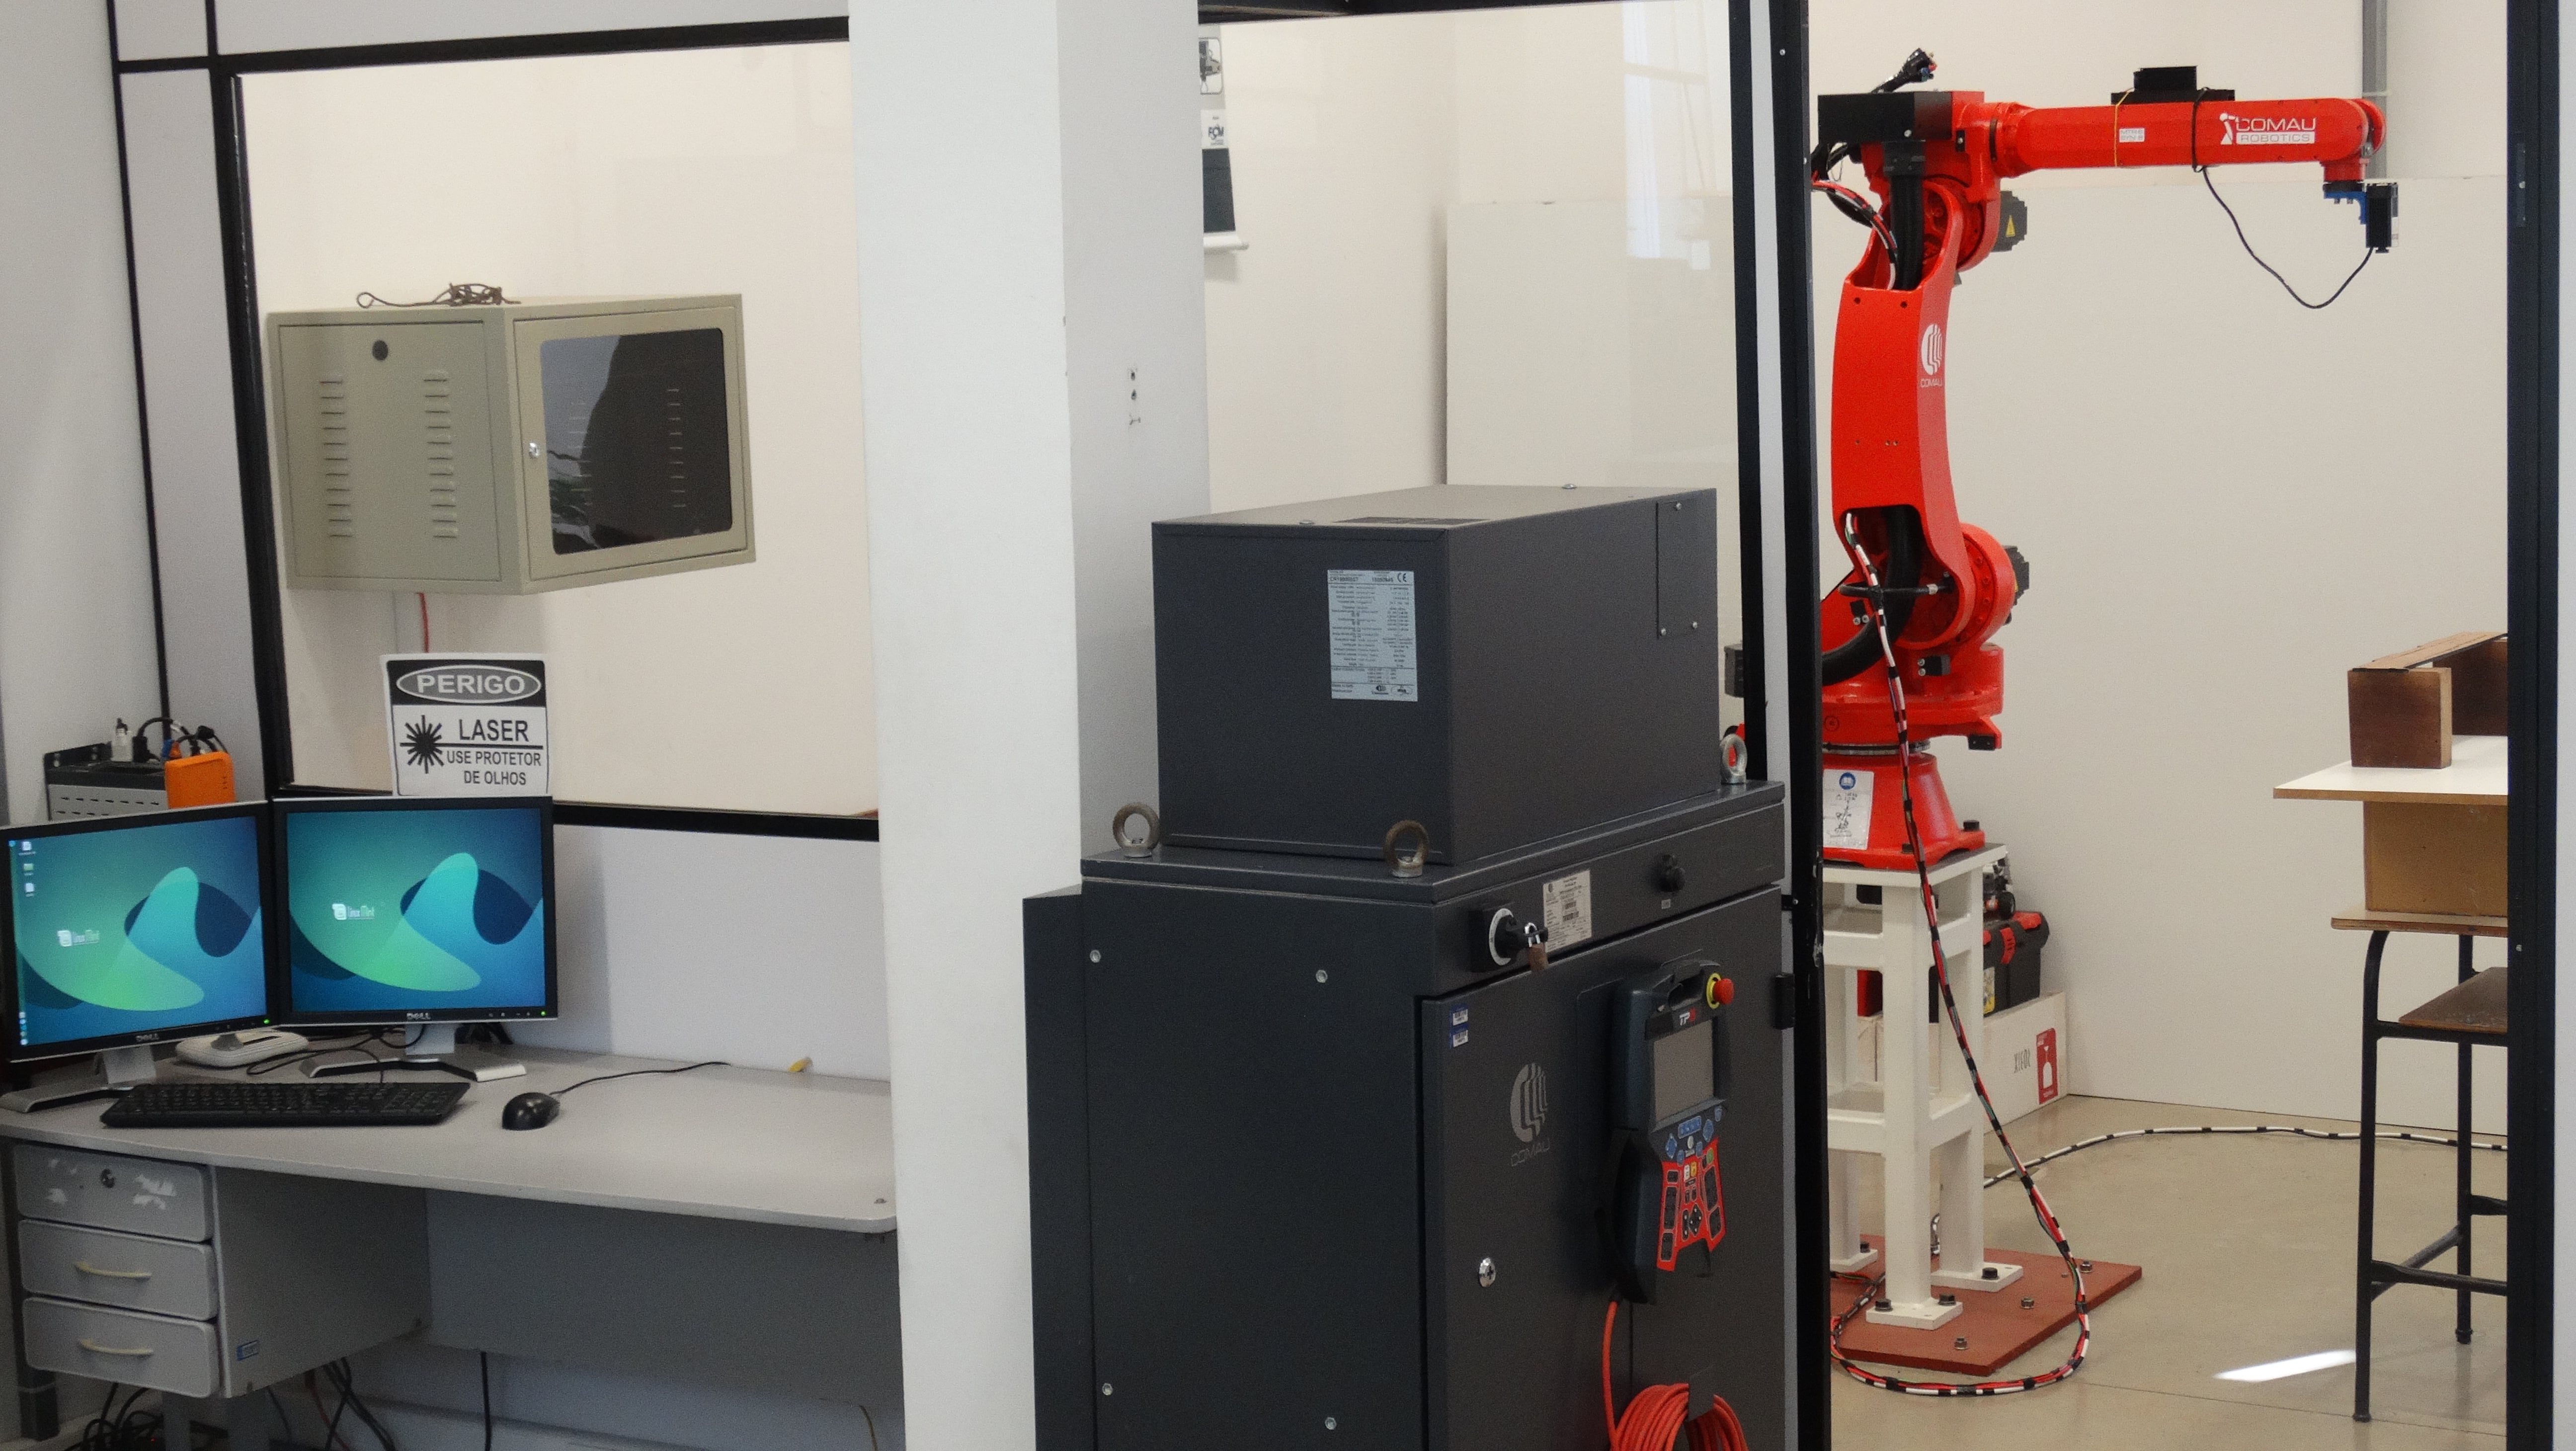
\includegraphics[width=\columnwidth]{imagens/Fotos/estrutura-lab-1.JPG}
        \small 
        \centering 
        \caption{Estrutura do laboratório onde será executado o OpenServer}
        \label{lab1}
    \end{figure}
    
    Estão disponíveis dois computadores para a execução de programas cliente, que podem ser vistos na Figura~\ref{lab2}, conectados à rede interna.
    
    \begin{figure}[ht]
        \centering
        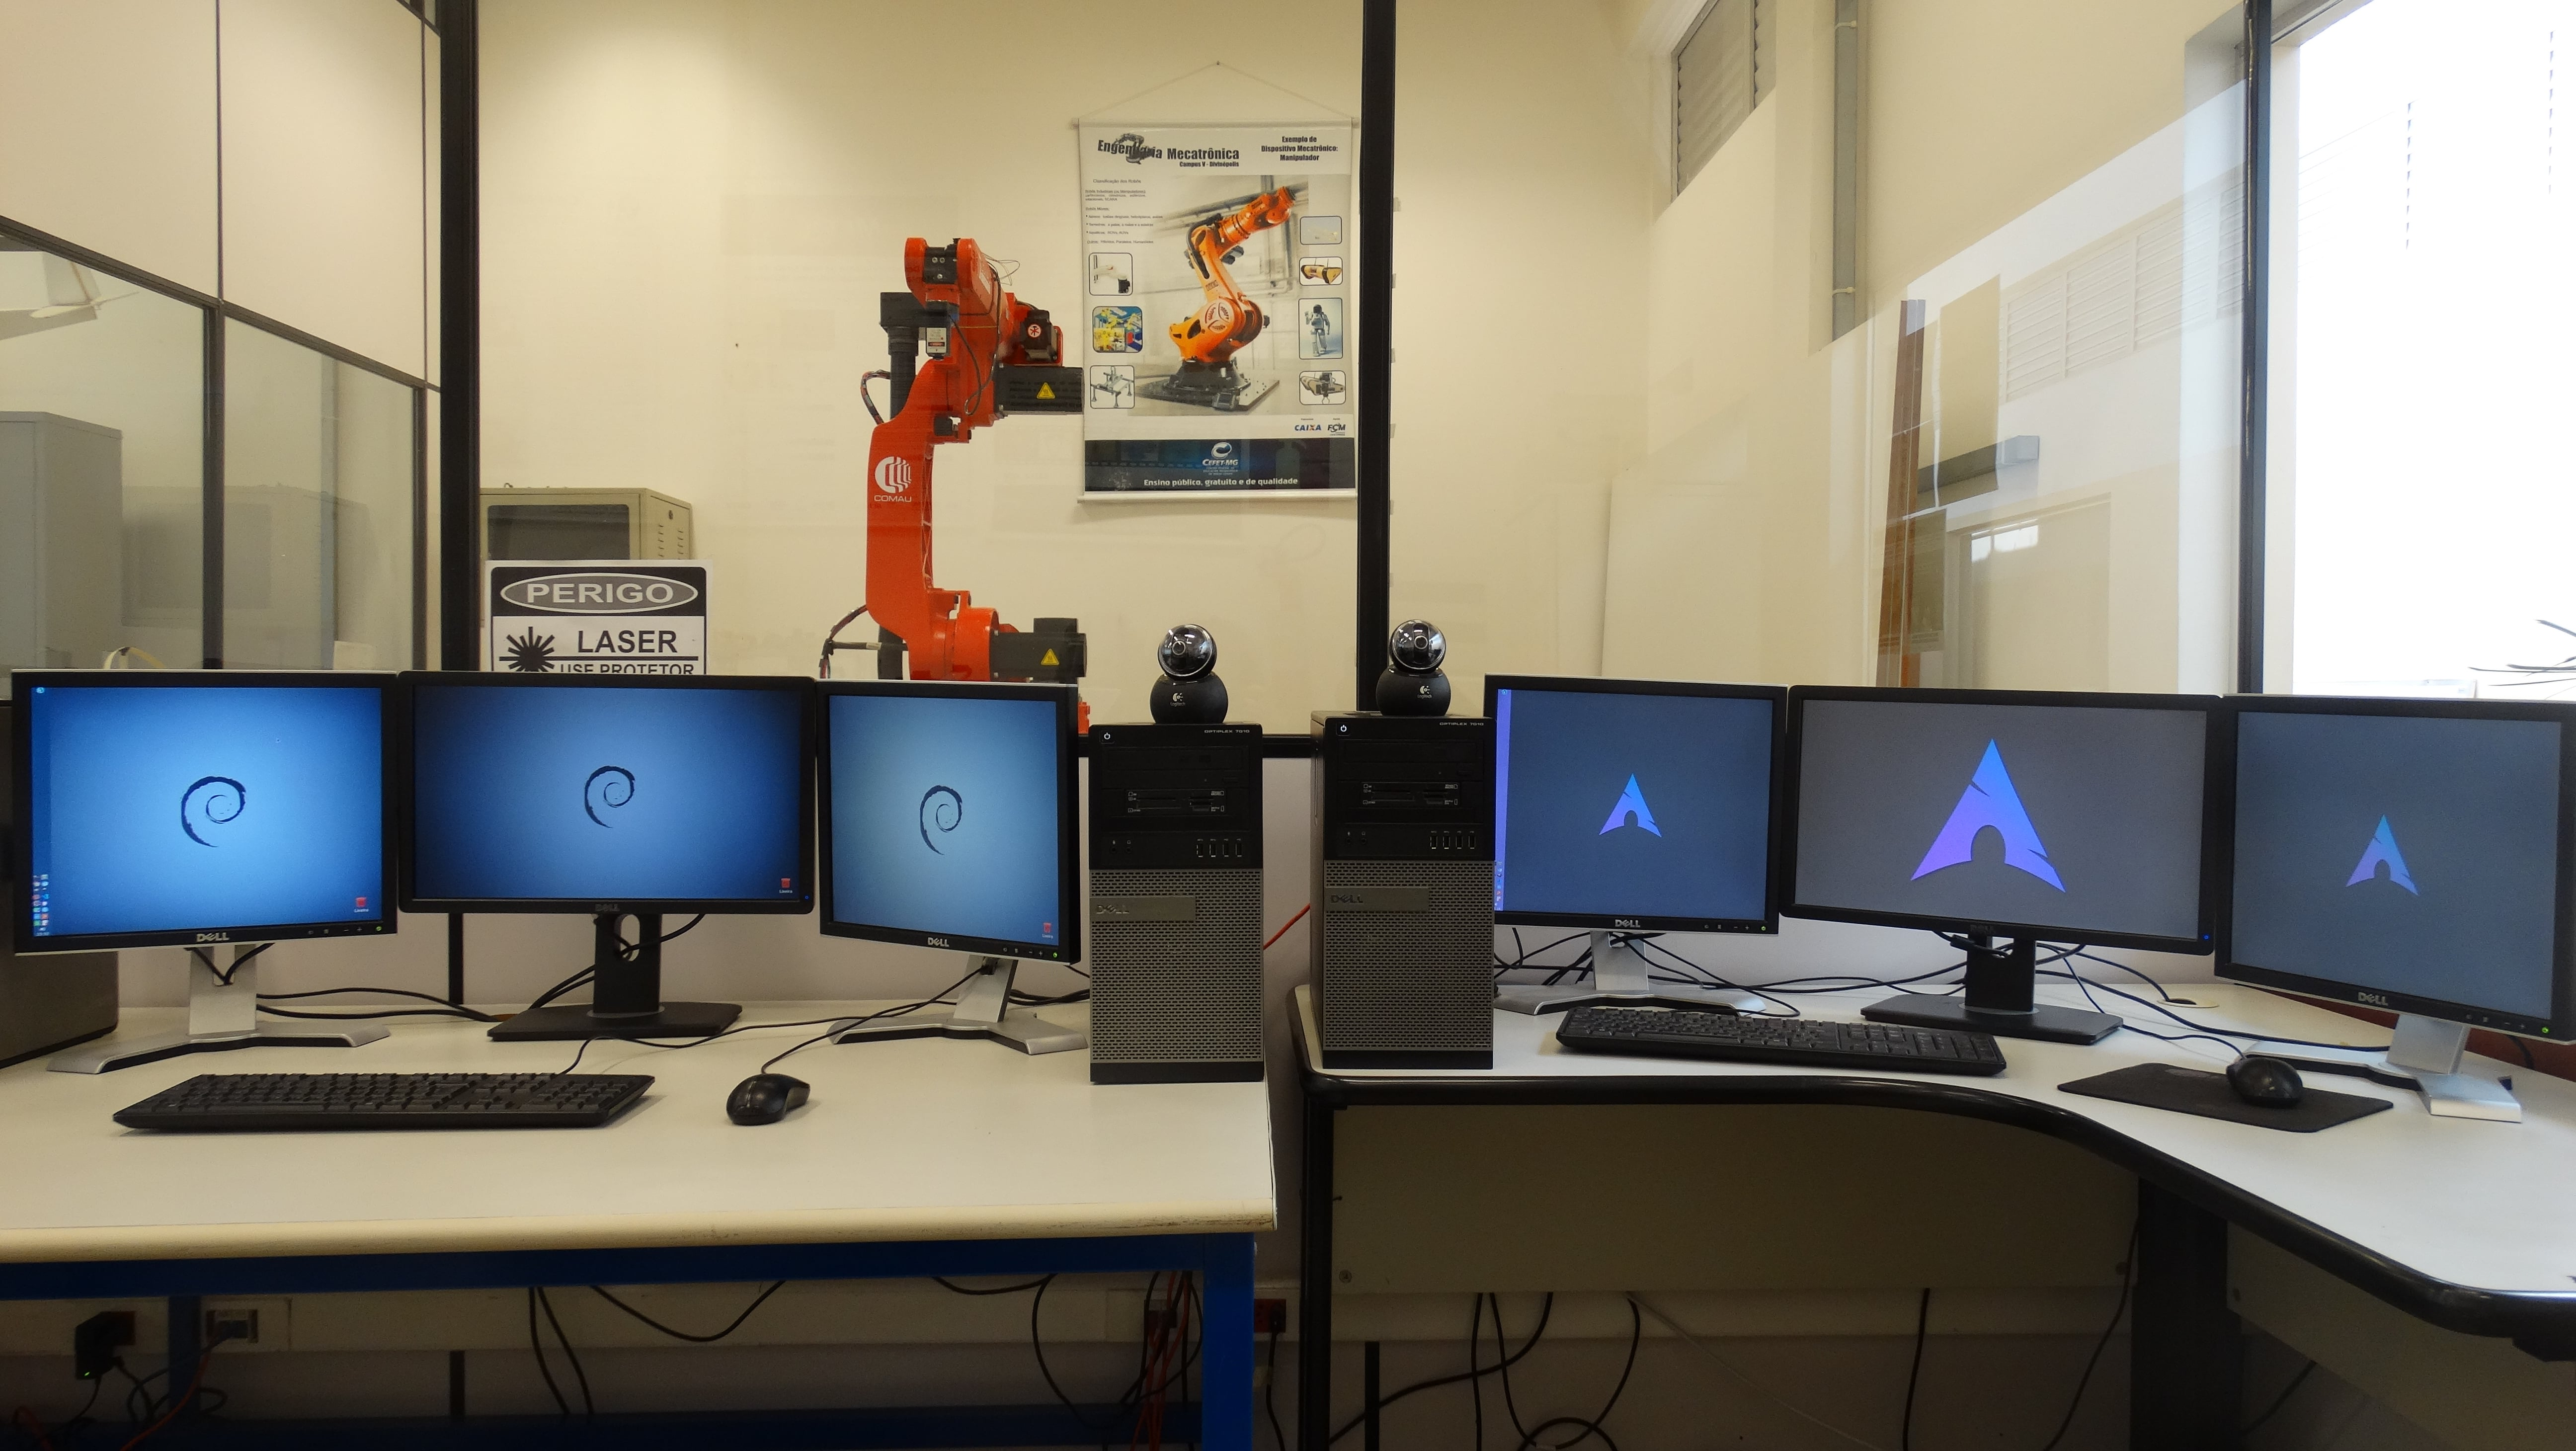
\includegraphics[width=\columnwidth]{imagens/Fotos/estrutura-lab-2.JPG}
        \small 
        \centering 
        \caption{Estrutura do laboratório onde será executado o OpenServer}
        \label{lab2}
    \end{figure}
        
    Para utilizar o sistema \textit{Open} é crucial a instalação da biblioteca \textit{eORL} no \textit{LPC} na mesma versão da \textit{eORL} da controladora~\citep{Open:Manual}. No caso, essa biblioteca já estava instalada no LPC, sendo necessária apenas a atualização dela para a última versão estável. Além disso, quando se desejar usar o sistema Open, é necessário habilitar o modo Open nos eixos desejados dentro do programa \textit{Crcopen}, conforme indicado na Figura~\ref{habilitar-open}.
    
    \begin{figure}[ht]
        \centering
        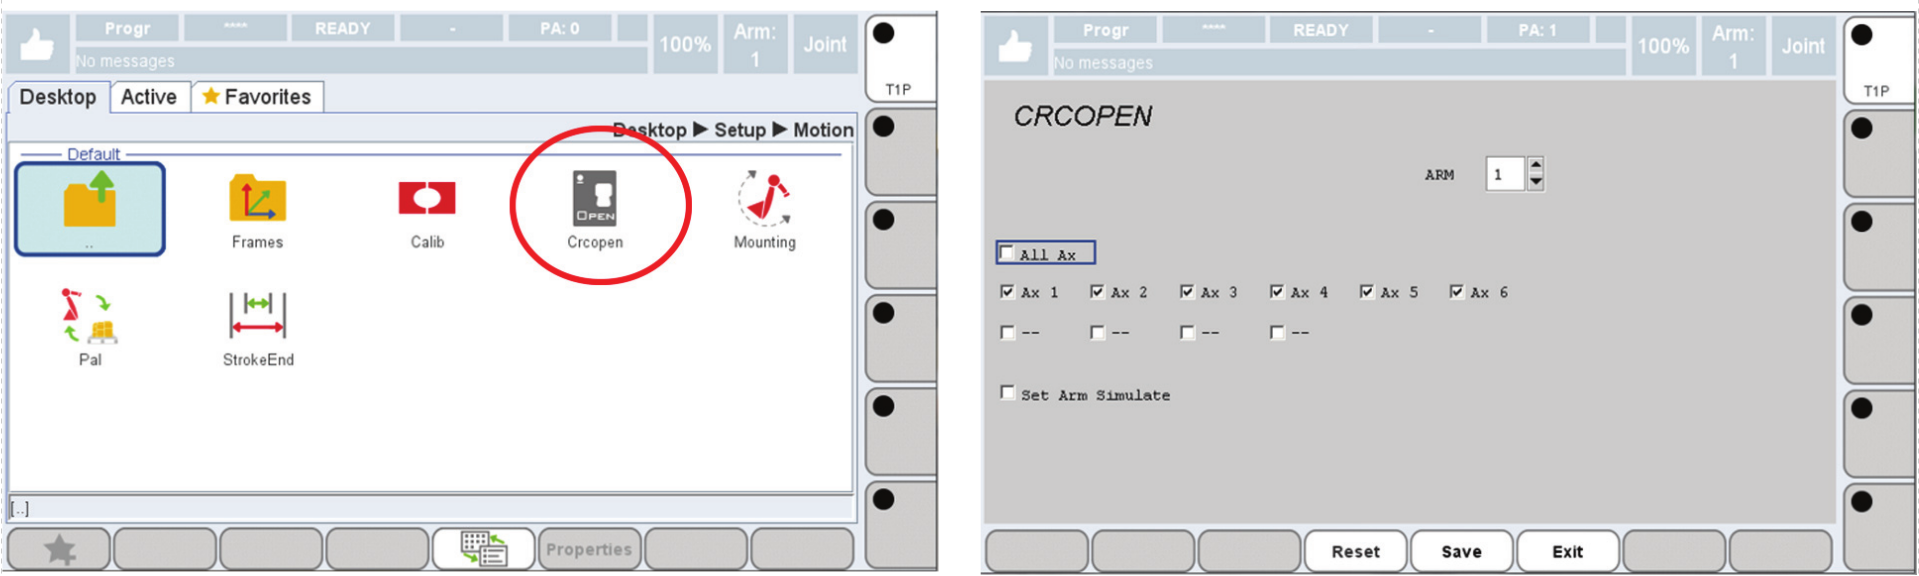
\includegraphics[width=\columnwidth]{imagens/Softwares/habilitar-open.png}
        \small 
        \centering 
        \caption{Procedimento para habilitar o modo Open dos eixos do robô~\citep{Open:Manual}}
        \label{habilitar-open}
    \end{figure}
    
    O desenvolvimento deste software torna mais segura a utilização do sistema Open em um ambiente de ensino e pesquisa, pois, o único software que precisará ser executado no \textit{LPC} passa a ser o \textit{OpenSever} em sua versão estável. Já no dispositivo externo serão executados os softwares experimentais, em desenvolvimento, os quais podem travar durante a execução. Quando isso acontece, o \textit{OpenSever} continua sendo executado no \textit{LPC} e comunicando com a controladora do robô, enviando a última referência armazenada. Dessa forma, o risco de se interromper bruscamente a comunicação com a controladora é evitado.
    
    Além disso, o \textit{OpenSever} expõe apenas um subconjunto das funcionalidades e configurações da \textit{eORL}, simplificando a utilização e reduzindo a quantidade de erros possíveis.
    
    \subsection{Funcionamento}
    
        Foi implementado um modo \textit{DEBUG}, a ser ativado antes do processo de compilação que imprime no terminal qual função foi executada, o comando vindo do programa cliente e a resposta enviada, conforme pode ser visto nas Figuras~\ref{openserver-wait}, \ref{openserver-ok}~e~\ref{openserver-send}. Quando o modo \textit{DEBUG} não está ativado apenas a biblioteca \textit{eORL} imprime textos no terminal, por exemplo, a tela de boas vindas, mensagens de erro, entre outros.
        
        Quando o software é executado, ele tenta se conectar com a controladora usando a biblioteca \textit{eORL} através da rede \textit{Powerlink}. Quando a conexão é bem sucedida o software entra em modo \textit{Listen}, ou seja, fica esperando um cliente se conectar ao \textit{soket} através da rede TCP/IP via \textit{Ethernet}, conforme pode ser visto na Figura~\ref{openserver-wait}.
        
        \begin{figure}[ht]
            \centering
            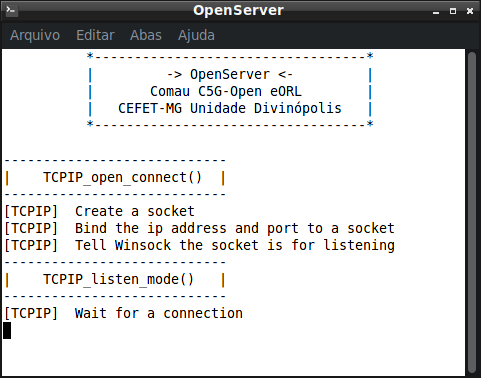
\includegraphics[width=\columnwidth]{imagens/Softwares/openserver-wait_.png}
            \small 
            \centering 
            \caption{OpenServer esperando a conexão de um \textit{software} cliente}
            \label{openserver-wait}
        \end{figure}
        
        Quando um cliente se conecta ao servidor é realizada uma troca de pacotes para verificar a integridade da conexão. Caso essa verificação seja bem sucedida o servidor fica esperando o recebimento de instruções do cliente, conforme pode ser visto na Figura~\ref{openserver-ok}. O servidor só atua mediante os comandos do cliente.
        
        \begin{figure}[ht]
            \centering
            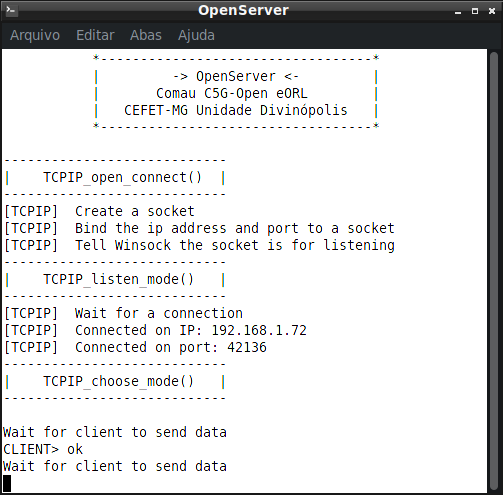
\includegraphics[width=\columnwidth]{imagens/Softwares/openserver-ok_.png}
            \small 
            \centering 
            \caption{OpenServer esperando a instrução do \textit{software} cliente conectado}
            \label{openserver-ok}
        \end{figure}
        
        O primeiro caractere recebido pelo servidor informa qual procedimento ele deve seguir. No caso, a instrução `p' é atualmente a instrução padrão. Ela está configurada para os valores de referência das juntas do robô (truncado em 5 casas decimais, mas, sem uso da vírgula para representar as casas decimais) virem concatenados na forma de \textit{strings} logo após tal instrução, como pode ser visto na Figura~\ref{openserver-send}. Ao receber essa instrução, imediatamente o servidor atualiza as variáveis de referência das juntas do robô na biblioteca \textit{eORL}, as quais são enviadas para a controladora. Em seguida, também na forma concatenada sem uso de virgula, o servidor envia a resposta ao programa cliente com a leitura mais recente dos sensores das juntas do robô armazenada na memória do servidor, as quais, foram recebidas da controladora aberta.
        %Logo em seguida, a controladora envia a resposta ao programa cliente com os valores atuais dos sensores das juntas do robô, também na forma concatenada sem uso de virgula. 
        
        \begin{figure}[ht]
            \centering
            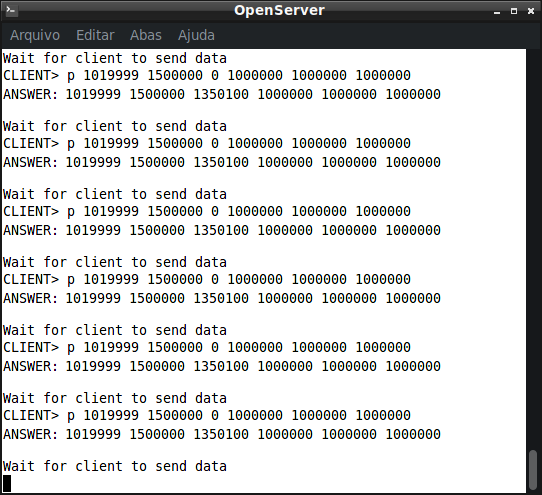
\includegraphics[width=\columnwidth]{imagens/Softwares/openserver-send_.png}
            \small 
            \centering 
            \caption{OpenServer executando a instrução do \textit{software} cliente e respondendo com a leitura dos sensores}
            \label{openserver-send}
        \end{figure}
        
        Esta forma de transmitir os dados (\textit{strings} concatenadas) foi desenvolvida com a intenção de ser uma construção simples de ser implementada em outras linguagens de programação.

        Como as taxas de transmissão de dados podem não ser necessariamente as mesmas, foi implementado um algoritmo interno que resolve esse problema de falta de sincronia. Por exemplo, a taxa de comunicação da \textit{eORL} com a controladora varia de uma taxa de $0,4\,\mathrm{ms}$ a $16\,\mathrm{ms}$; e a taxa de comunicação entre o programa servidor e o programa cliente não tem uma faixa definida. Assim, o desenvolvedor do programa cliente tem a liberdade de programar a taxa que for mais conveniente (dentro dos limites práticos da rede) e, inclusive, enviar os comandos de movimentação de forma não constante.
        
    \section{Resultados e Discussões}
    
    Para testar o servidor foi preciso desenvolver um software cliente que se comunique com ele via rede TCP/IP, o qual, permite o usuário enviar os ângulos de referência de cada junta do robô e visualizar as leituras dos sensores de posição angular (\textit{encoder} absoluto de precisão) de cada junta em tempo real. 
    
    \begin{figure}[H]
        \centering
        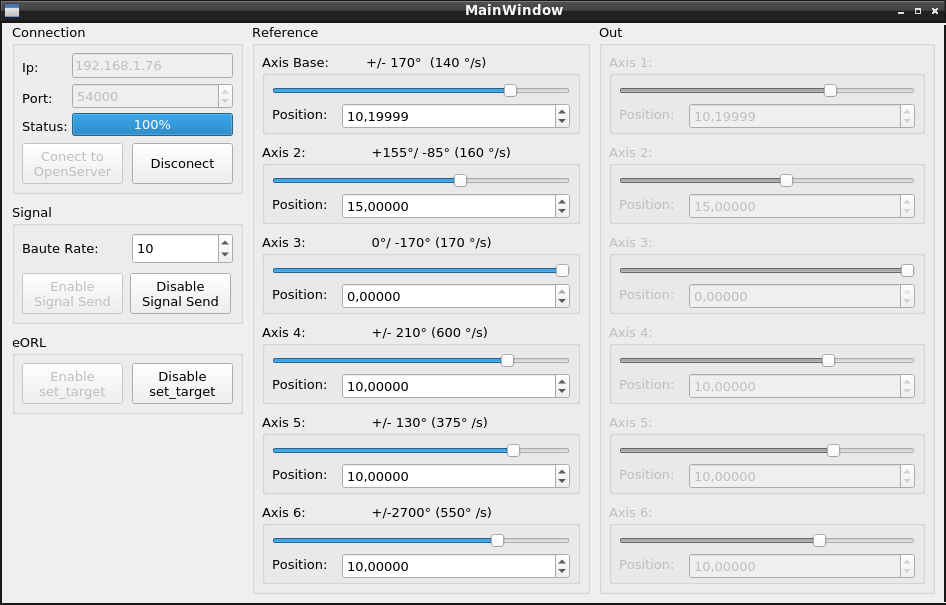
\includegraphics[width=\columnwidth]{imagens/Softwares/openclient_.png}
        \small 
        \centering 
        \caption{Software OpenClient em execução}
        \label{openclient_}
    \end{figure}
    
    Tal software foi chamado de \textit{OpenClientExemple}, escrito em C++ usando bibliotecas padrão do sistema operacional baseado em Linux, mas, que pode ser compilado para a arquitetura \textit{x86-64}, tendo sido executado em um computador pessoal convencional. Ele foi compilado também para \textit{Arm64} e executado em um \textit{Raspberry Pi 4}. Ambos testes foram realizados com sucesso, demonstrando que podem ser desenvolvidos programas clientes em outras arquiteturas.
    
    Além disso, foi testada a comunicação com o software \textit{Python}, usando a biblioteca padrão TCP/IP do mesmo, sendo executado no Sistema Operacional \textit{Windows} e também testada com um dispositivo móvel rodando \textit{Android}. A comunicação com o OpenServer foi realizada com sucesso, demonstrando que podem ser desenvolvidos softwares clientes em outros sistemas operacionais, inclusive para dispositivos móveis.
    
    A taxa de comunicação de um pacote a cada $2\,\mathrm{ms}$ (um pacote contendo todas as leituras ou posições das juntas), que foi aferida via cabo pode ser o suficiente para a maioria das aplicações, mas, essa taxa pode ser melhorada desenvolvendo-se uma forma mais eficiente de transmitir os dados. Por exemplo, criando uma nova modalidade que, de forma síncrona, envie dados ao mesmo tempo que recebe, ao invés de usar a forma assíncrona, que aguarda o recebimento de um dado para enviar o próximo. Outra possibilidade seria criar outra modalidade em que sejam transmitidos os dados binários direto da memória RAM, ao invés de convertê-los em \textit{strings} como foi feito nesse trabalho.
    
    A comunicação via rede sem fio também ocorreu a uma taxa de $2\,\mathrm{ms}$, com exceção de quando ocorria perda de dados devido à distância.

    \section{Conclusões e Perspectivas}

    O presente trabalho teve como foco a expansão das possibilidades de recursos da controladora aberta \textit{C5G-Open} através da implementação de um sistema cliente servidor. Os resultados preliminares foram considerados satisfatórios, motivando a continuidade do desenvolvimento dos softwares e do projeto em si. A sub-rede demonstrou garantir a comunicação de forma estável e rápida. A integração dos softwares foi facilitada pela padronização do protocolo TCP/IP, o que ajudou expandir as possibilidades de uso do OpenServer.
    
    A perspectiva futura é usar o OpenSever para dar início ao desenvolvimento de malhas de controle adicionais ao sistema robótico como uma malha de visão computacional. Uma câmera afixada no efetuador do robô filmará uma figura de referência, o software cliente processará a imagem e gerará os comandos de movimentação que serão enviados ao OpenServer, de forma a manter constante a pose (posição e orientação) do manipulador robótico em relação à pose da figura de referência. Dessa maneira, deverá ser adicionada uma câmera à estrutura desenvolvida, conforme pode ser visto na Figura~\ref{pespectiva}, onde (1) representa a câmera; e (2) a figura de referência.
    
    
    \begin{figure}[ht]
        \centering
        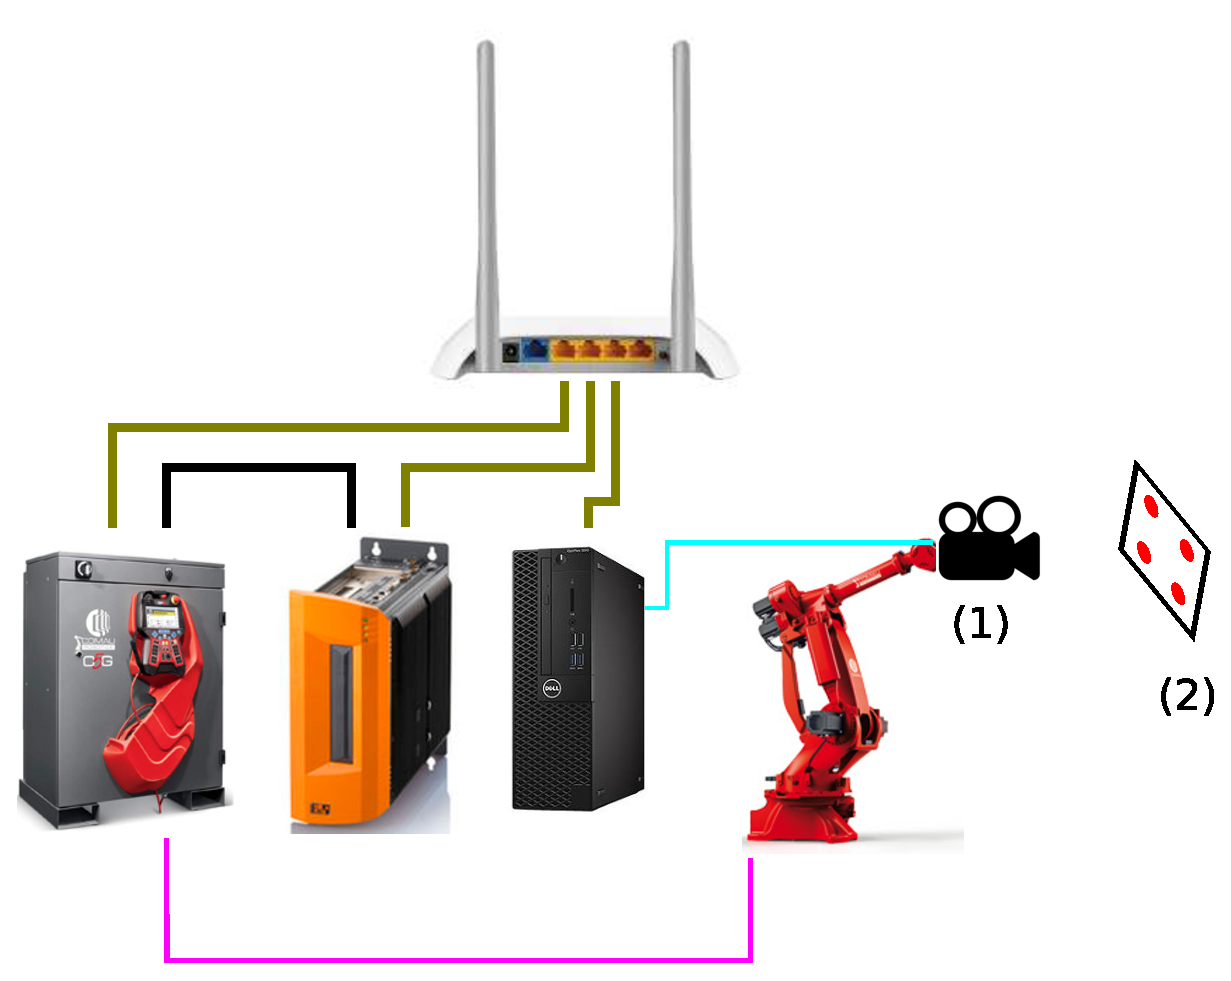
\includegraphics[width=\columnwidth]{imagens/pespectiva.eps}
        \small 
        \centering 
        \caption{Estrutura proposta para utilização do OpenServer}
        
        \label{pespectiva}
    \end{figure}
    
\section{Agradecimentos}
    %E o CEFET-MG ?
    Agradecemos ao CNPq - Conselho Nacional de Desenvolvimento Científico e Tecnológico - pelo apoio financeiro dado a essa pesquisa através da concessão de bolsa do PIBTI - Programa Institucional de Bolsas de Desenvolvimento Tecnológico e Inovação. Agradecemos também a COMAU Robotics pelo suporte técnico e orientações dadas.
    %\nocite{*}
    \bibliography{6-referencias}

\end{document}
